\documentclass[10pt, aspectratio=169]{beamer}
\usetheme{Madrid}
\usecolortheme{dolphin}
\usepackage[utf8]{inputenc}
\usepackage{amsmath,amssymb,amsthm,mathtools}
\usepackage{graphicx}
\usepackage{booktabs}
\usepackage{hyperref}
\usepackage{url}

% --- Font Settings ---
\usepackage{newtxtext,newtxmath}

% --- Remove navigation symbols ---
\setbeamertemplate{navigation symbols}{}

% --- Title and Author ---
\title[Seasonal Trading Strategies]{Seasonal Trading Strategies: Identifying Optimal Entry and Exit Windows across NEPSE Sub-Sectors}
\author[Tek Raj Pant, Himal Jung Oli]{Tek Raj Pant \and Himal Jung Oli \\ M.Sc. Computational Mathematics \\ Computational Statistics}
\institute[Kathmandu University]{Department of Mathematics \\ School of Science \\ Kathmandu University}
\date{June 2026}

% --- Logo on every slide ---

\begin{document}

% ------------------- TITLE PAGE -------------------
\begin{frame}
\titlepage
\end{frame}

% ------------------- OUTLINE -------------------
\begin{frame}{Outline}
\tableofcontents
\end{frame}

% ===============================================================
%  SECTION 1: Introduction  (Slide 1)
% ===============================================================
\section{Introduction}

\begin{frame}{Introduction}
\begin{itemize}
    \item The Nepal Stock Exchange (NEPSE) often exhibits patterns influenced by the Bikram Sambat calendar, fiscal year cycles, and major festivals like Dashain and Tihar \cite{shrestha2023seasonal}.
    \item This project explores the \textit{Seasonality Hypothesis} --- stock returns are not purely random but follow periodic trends that challenge weak-form efficiency \cite{joshi2025broad}.
    \item By analysing sectoral performance over five years (2021--2026), we distinguish genuine anomalies from noise \cite{basnet2022efficient}.
    \item Different sub-sectors show unique trends tied to fiscal year closings and festive windows \cite{gurung2024fiscal}. Our goal: identify optimal entry and exit windows using historical data \cite{adhikari2024calendar, sharma2021investor}.
\end{itemize}
\end{frame}

% ===============================================================
%  SECTION 2: Objectives  (Slide 2)
% ===============================================================
\section{Objectives}

\begin{frame}{Objectives}
\begin{enumerate}
    \item Identify statistically significant monthly/seasonal trends within NEPSE sub-sectors.
    \item Quantify risk-return profiles during high-volatility periods.
    \item Develop a Z-score based entry--exit framework for optimising trading timing.
\end{enumerate}
\end{frame}

% ===============================================================
%  SECTION 3: Data Source  (Slide 3)
% ===============================================================
\section{Data Source}

\begin{frame}{Data Source}
\begin{itemize}
    \item \textbf{Period:} 2021 -- 2026 (daily closing prices).
    \item \textbf{Source:} Nepse Alpha (\url{https://nepsealpha.com/nepse-data}).
    \item \textbf{Sectors covered:} Banking, Hydropower, Manufacturing, Microfinance, Non-Life Insurance, Others.
    \item Daily returns are computed as:
    \[
    R_t = \frac{P_t^{\text{close}} - P_{t-1}^{\text{close}}}{P_{t-1}^{\text{close}}}
    \]
    where $P_t^{\text{close}}$ denotes the closing price at time $t$.
\end{itemize}
\end{frame}

% ===============================================================
%  SECTION 4: Methodology  (Slides 4--5)
% ===============================================================
\section{Methodology}

\begin{frame}{Methodology -- Exploratory \& Distributional Analysis}
\begin{itemize}
    \item \textbf{Boxplots} \cite{tukey1977eda}: IQR-based outlier detection across sectors.
    \item \textbf{Histograms \& Q--Q plots} \cite{chambers1983graphical}: assess normality departures.
    \item \textbf{Skewness} \cite{joanes1998comparing}: $g_1 = \frac{1}{n}\sum\!\bigl(\frac{x_i-\bar{x}}{s}\bigr)^{\!3}$\,.
    \item \textbf{Excess kurtosis} \cite{de1992tests}: $g_2 = \frac{1}{n}\sum\!\bigl(\frac{x_i-\bar{x}}{s}\bigr)^{\!4} - 3$\,.
    \item \textbf{Shapiro--Wilk test} \cite{shapiro1965variance}: formal normality test.
    \item \textbf{Additional EDA}: monthly bar charts with bootstrap CIs, density plots with normal reference, cumulative time-series, heatmap of sector$\times$month returns, ACF plots.
\end{itemize}
\end{frame}

\begin{frame}{Methodology -- Confirmatory \& Seasonality Detection}
\begin{columns}[T]
\column{0.48\textwidth}
\textbf{Hypothesis Tests}
\begin{itemize}
    \item Chi-square independence \cite{pearson1900chi}
    \item One-way ANOVA (month \& sector) \cite{fisher1925statistical}
    \item Two-way ANOVA (Sector$\times$Month) \cite{kutner2005applied}
    \item Kruskal--Wallis \cite{kruskal1952use}
    \item Mann--Whitney $U$ \cite{mann1947test}
\end{itemize}
\column{0.48\textwidth}
\textbf{Seasonality Detection}
\begin{itemize}
    \item Monthly ranking metrics (mean, Sharpe \cite{sharpe1966mutual}, win ratio)
    \item Z-score entry/exit framework \cite{tsay2010analysis}
    \item Cumulative return by day-of-year
    \item Year-on-year consistency \cite{lakonishok1988seasonal}
    \item Bootstrap CIs \cite{efron1994introduction}
    \item Robust ANOVA (trimmed means) \cite{wilcox2017introduction}
    \item Permutation test \cite{good2005permutation}
\end{itemize}
\end{columns}
\vspace{0.3cm}
\small\textbf{Regression:} Simple linear trend and autoregressive model ($R_t = \beta_0 + \beta_1 R_{t-1} + \beta_2\,\text{Sector} + \varepsilon_t$) \cite{draper1998applied}.
\end{frame}

% ===============================================================
%  SECTION 5: Results and Discussion  (Slides 6--19)
% ===============================================================
\section{Results and Discussion}

% --- Slide 6: Boxplot ---
\begin{frame}{EDA -- Boxplot of Closing Prices}
\begin{figure}
\centering
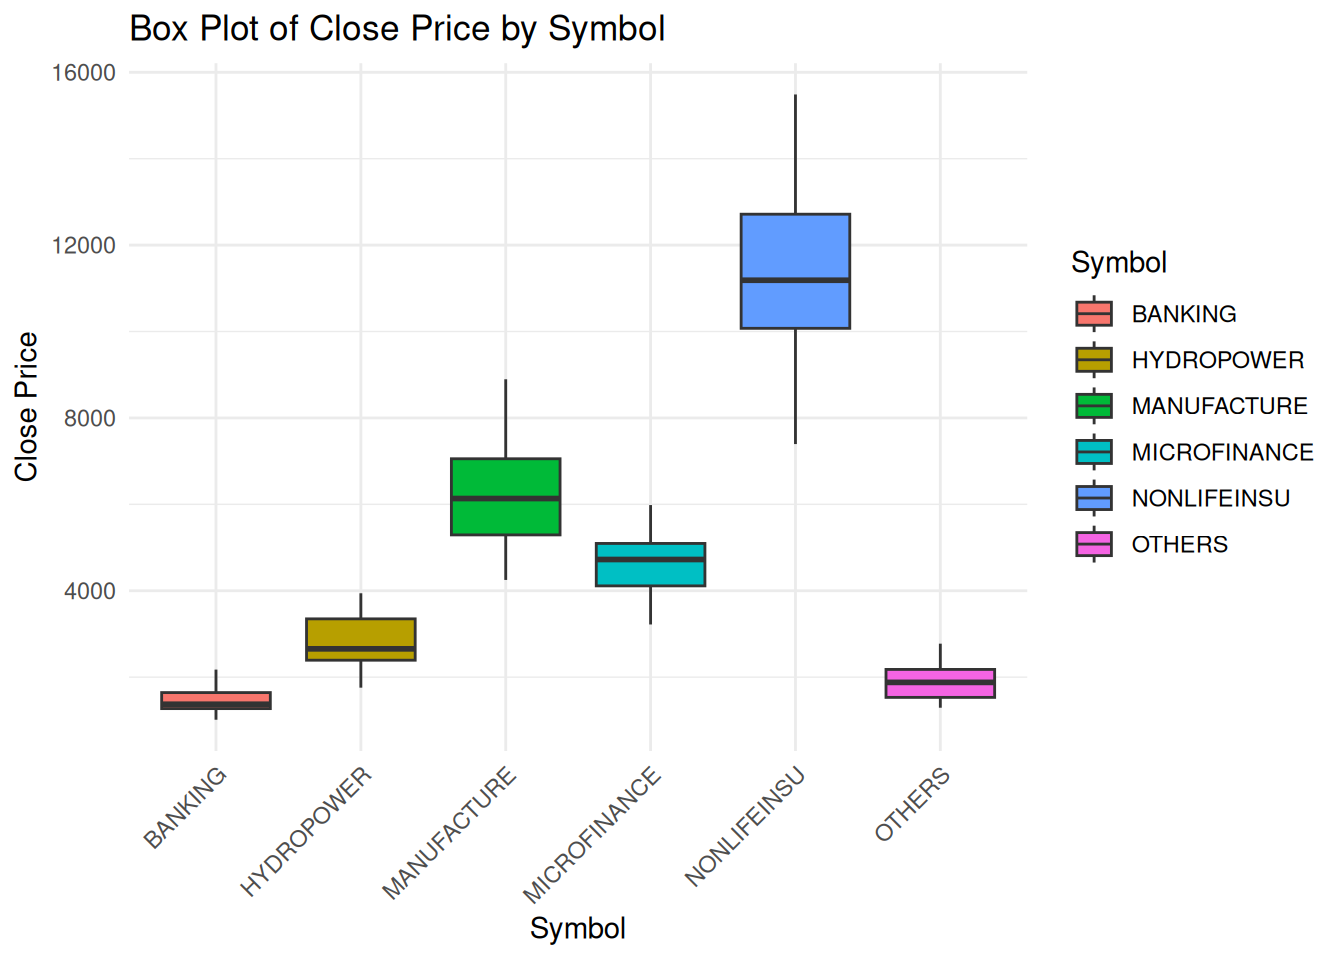
\includegraphics[width=0.78\textwidth]{figures/stats-box-plot.png}
\caption{Box plots of closing prices by sector. Outliers beyond $1.5\times\text{IQR}$.}
\end{figure}
\begin{itemize}
    \item Wide price ranges; Hydropower and Others show higher dispersion.
    \item Mild positive skewness in several sectors.
\end{itemize}
\end{frame}

% --- Slide 7: Q-Q Plots ---
\begin{frame}{EDA -- Q--Q Plots}
\begin{figure}
\centering
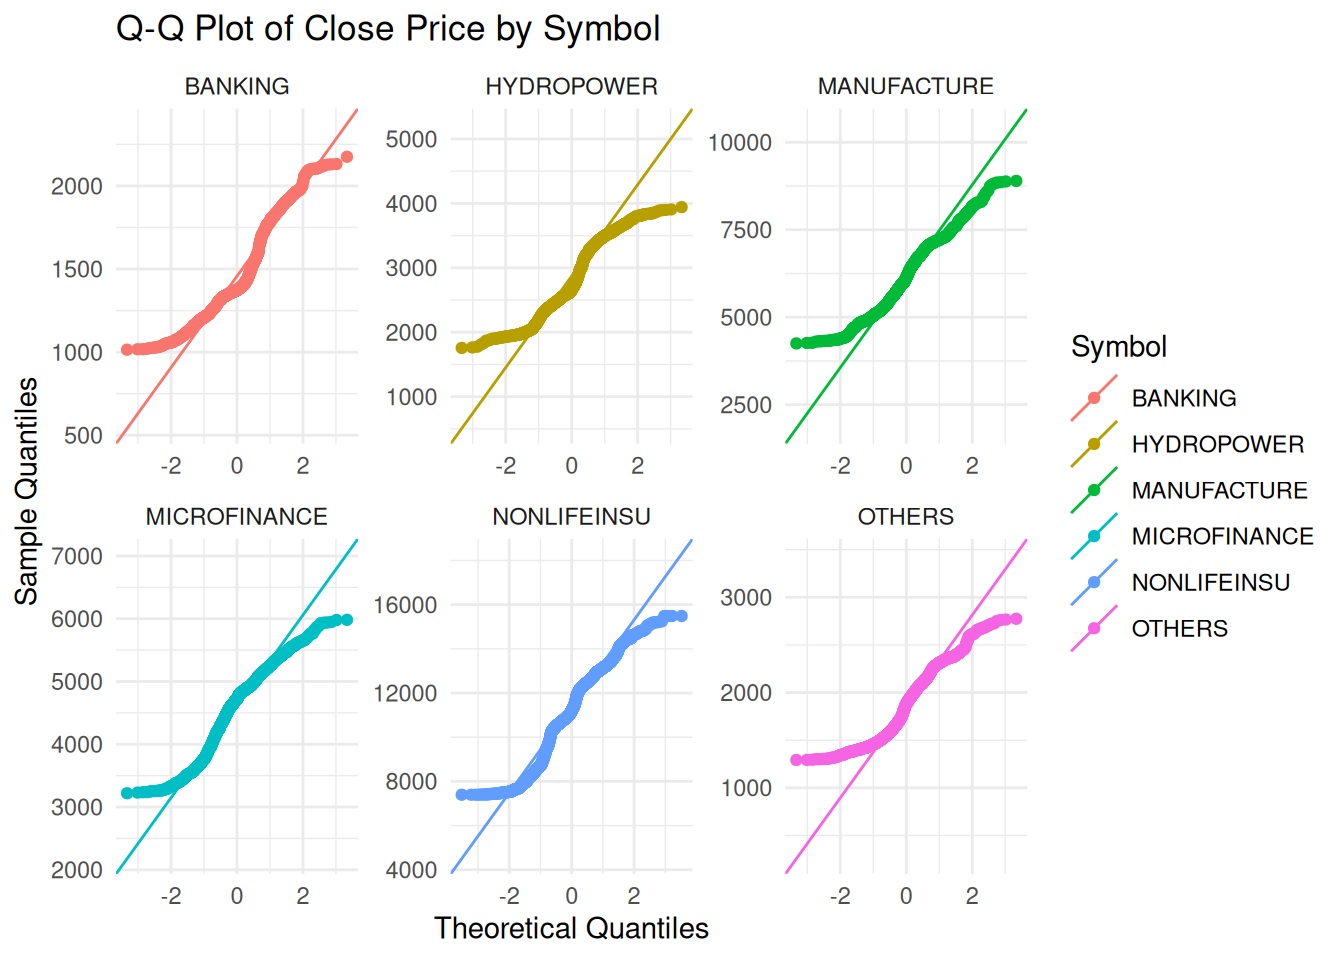
\includegraphics[width=0.78\textwidth]{figures/stats-q-q-plot.png}
\caption{Q--Q plots by sector. Deviations from the diagonal indicate non-normality.}
\end{figure}
\begin{itemize}
    \item All sectors exhibit heavy tails, especially at extremes.
    \item Strong visual evidence against normality.
\end{itemize}
\end{frame}

% --- Slide 8: Distribution Table ---
\begin{frame}{Distribution of Daily Returns}
\begin{table}
\centering
\caption{Distributional characteristics of daily returns by sector}
\small
\begin{tabular}{lrrrr}
\toprule
Sector & Mean & SD & Skewness & Excess Kurtosis \\
\midrule
BANKING       & $-0.000117$ & 0.0132 & 1.140 & 8.24 \\
HYDROPOWER    & $\hphantom{-}0.000770$ & 0.0209 & 0.615 & 4.44 \\
MANUFACTURE   & $\hphantom{-}0.000458$ & 0.0162 & 0.798 & 4.83 \\
MICROFINANCE  & $\hphantom{-}0.000365$ & 0.0164 & 0.802 & 6.58 \\
NONLIFEINSU   & $\hphantom{-}0.000723$ & 0.0114 & 0.976 & 9.88 \\
OTHERS        & $\hphantom{-}0.000376$ & 0.0184 & 0.638 & 4.87 \\
\bottomrule
\end{tabular}
\end{table}
\begin{itemize}
    \item All sectors: positive skewness and high excess kurtosis $\Rightarrow$ fat tails \cite{cont2001empirical}.
    \item Shapiro--Wilk test rejects normality for all sectors ($p<10^{-12}$) \cite{shapiro1965variance}.
\end{itemize}
\end{frame}

% --- Slide 9: Monthly Bar ---
\begin{frame}{EDA -- Monthly Average Returns with Bootstrap CIs}
\begin{figure}
\centering
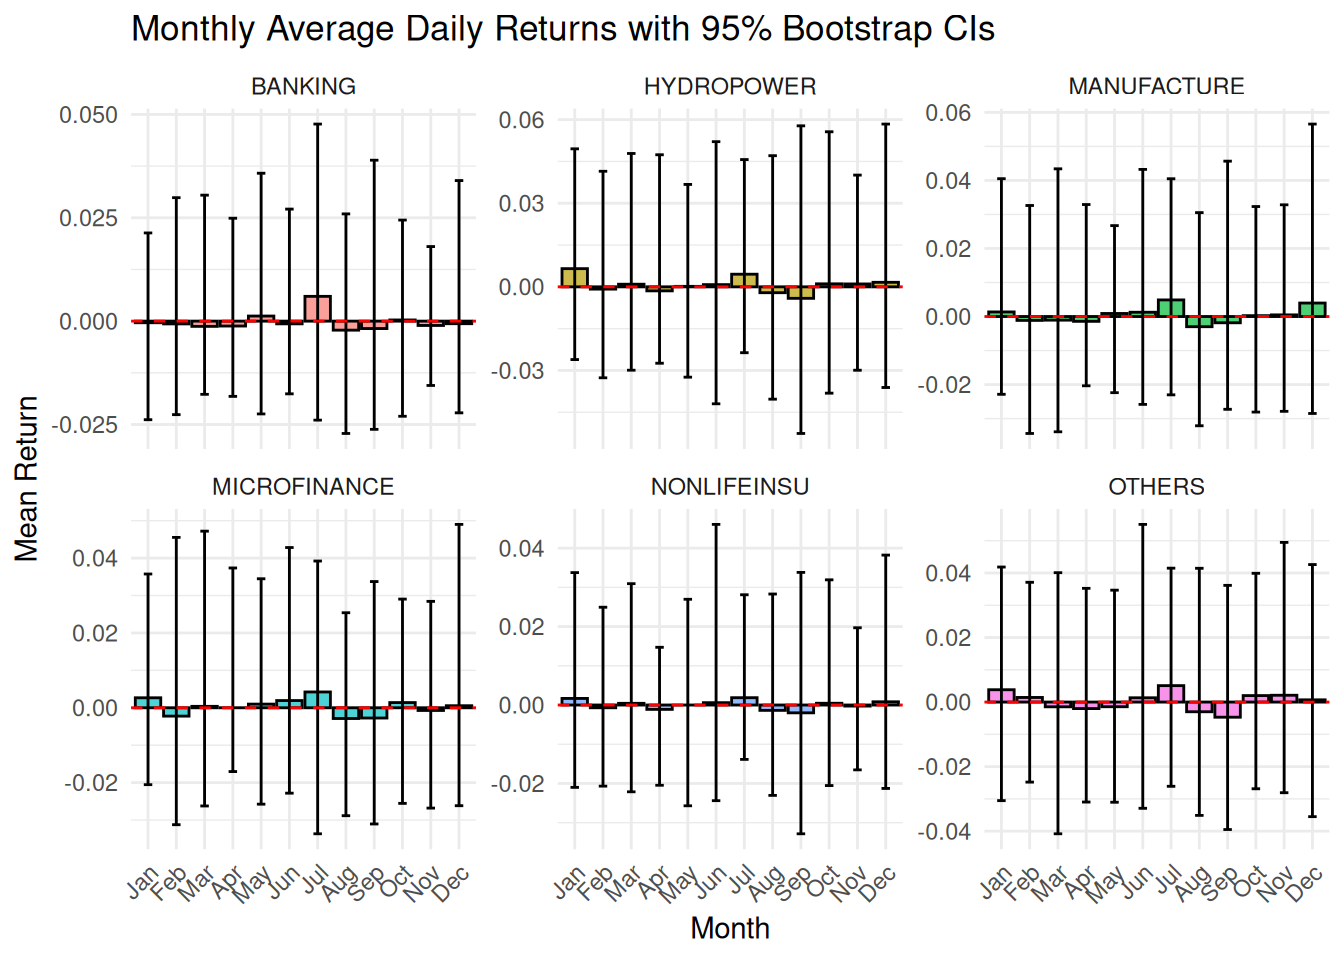
\includegraphics[width=0.82\textwidth]{figures/stats-monthly-bar.png}
\caption{Monthly average daily returns with 95\% bootstrap CIs. Red line = zero.}
\end{figure}
\begin{itemize}
    \item July (Shrawan) shows highest returns across all sectors.
    \item August--September consistently negative.
\end{itemize}
\end{frame}

% --- Slide 10: Density + Heatmap ---
\begin{frame}{EDA -- Return Density \& Heatmap}
\begin{columns}
\column{0.48\textwidth}
\begin{figure}
\centering
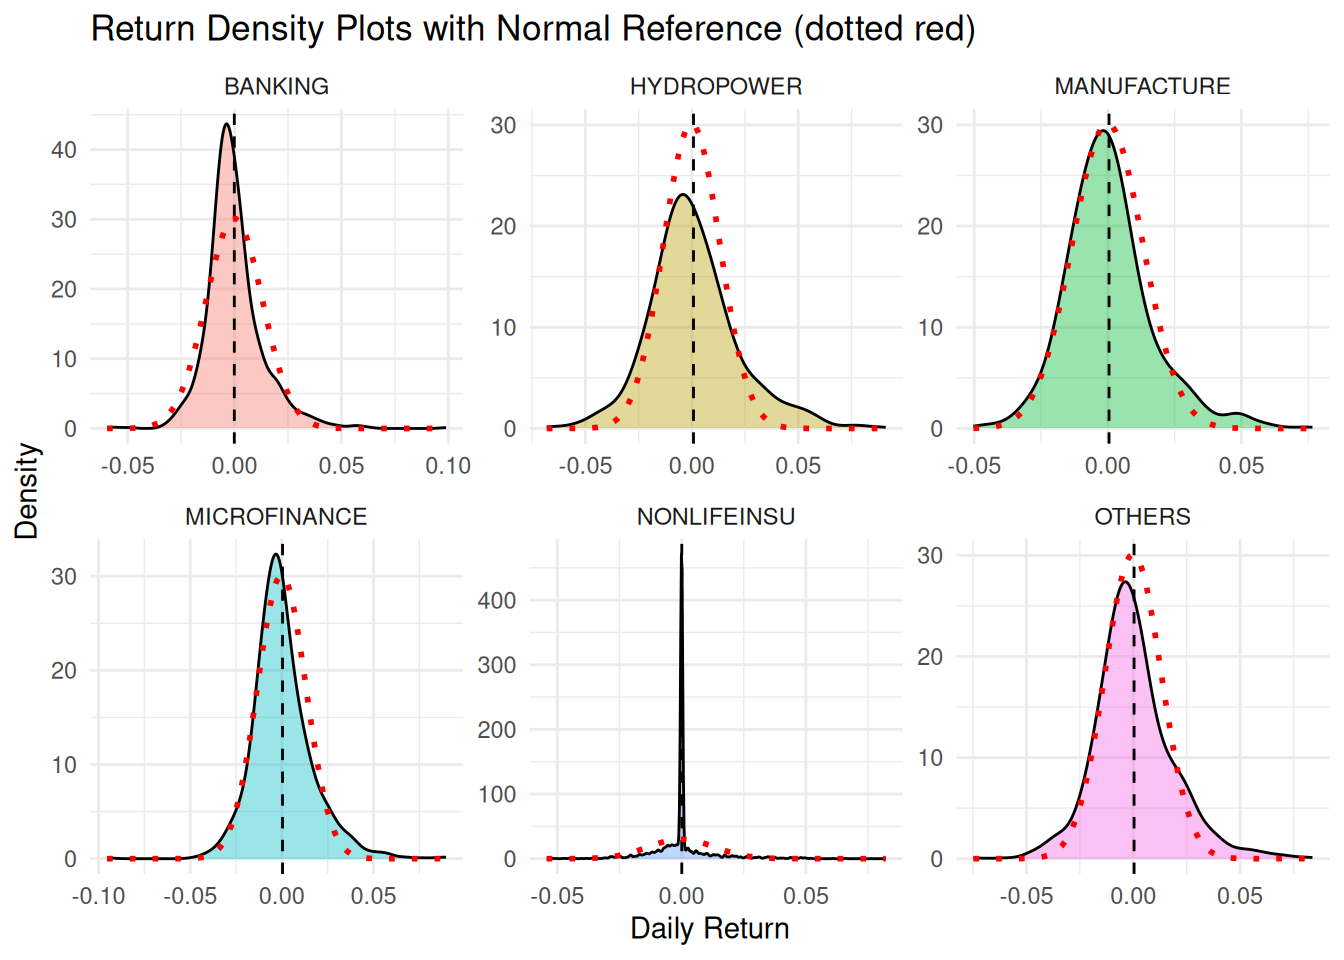
\includegraphics[width=\textwidth]{figures/stats-density.png.png}
\caption{Density plots with normal reference (dotted red).}
\end{figure}
\column{0.48\textwidth}
\begin{figure}
\centering
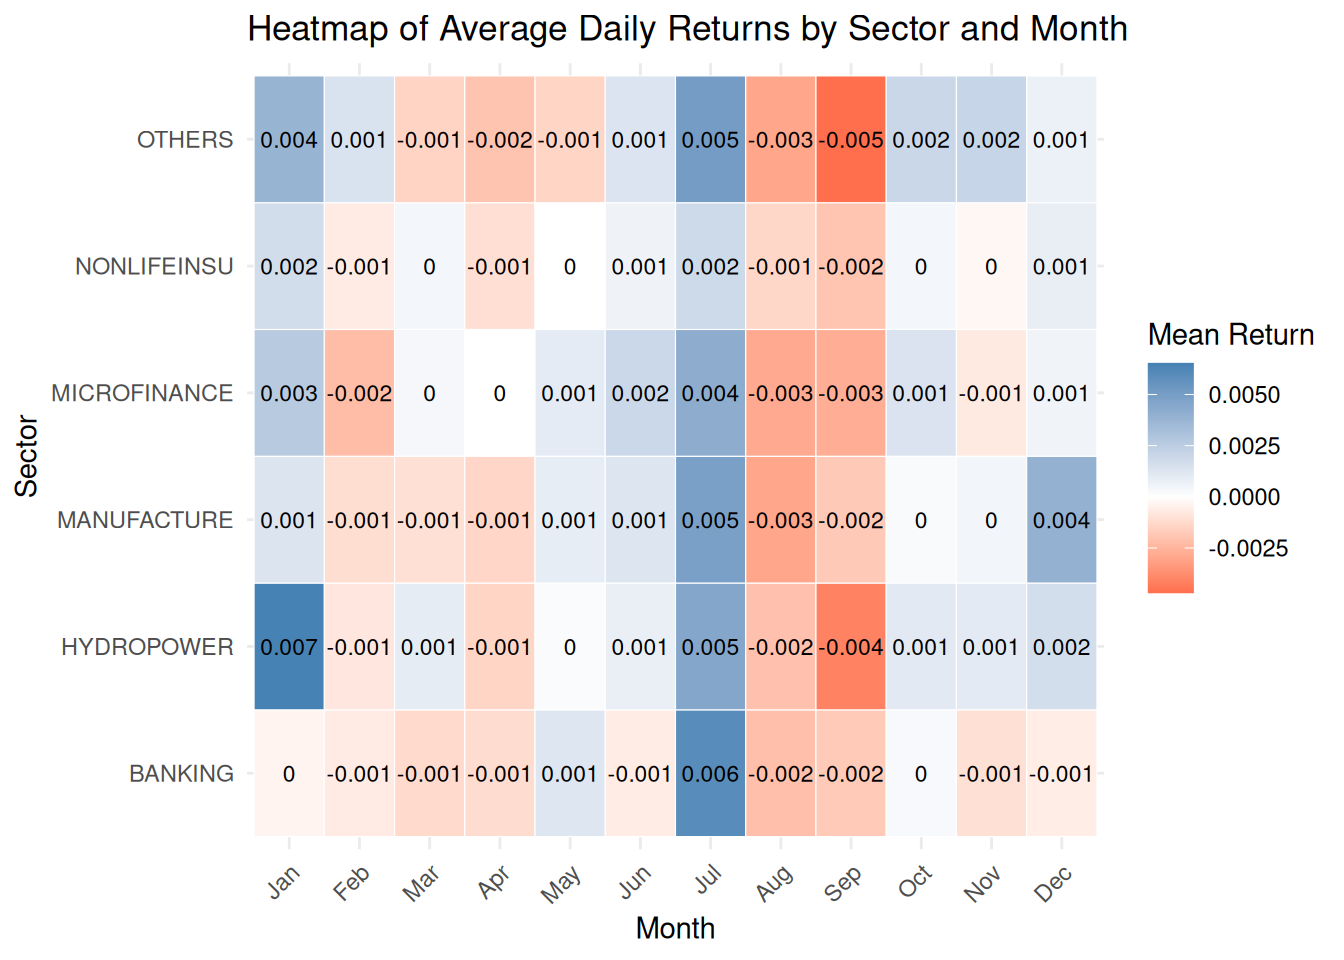
\includegraphics[width=\textwidth]{figures/stats-heatmap.png}
\caption{Heatmap: blue = positive, red = negative returns.}
\end{figure}
\end{columns}
\begin{itemize}
    \item Density plots confirm heavy tails and peakedness vs.\ normal.
    \item Heatmap highlights July as best, Aug--Sep as worst for all sectors.
\end{itemize}
\end{frame}

% --- Slide 11: Cumulative TS + Histogram ---
\begin{frame}{EDA -- Cumulative Returns \& Price Distribution}
\begin{columns}
\column{0.48\textwidth}
\begin{figure}
\centering
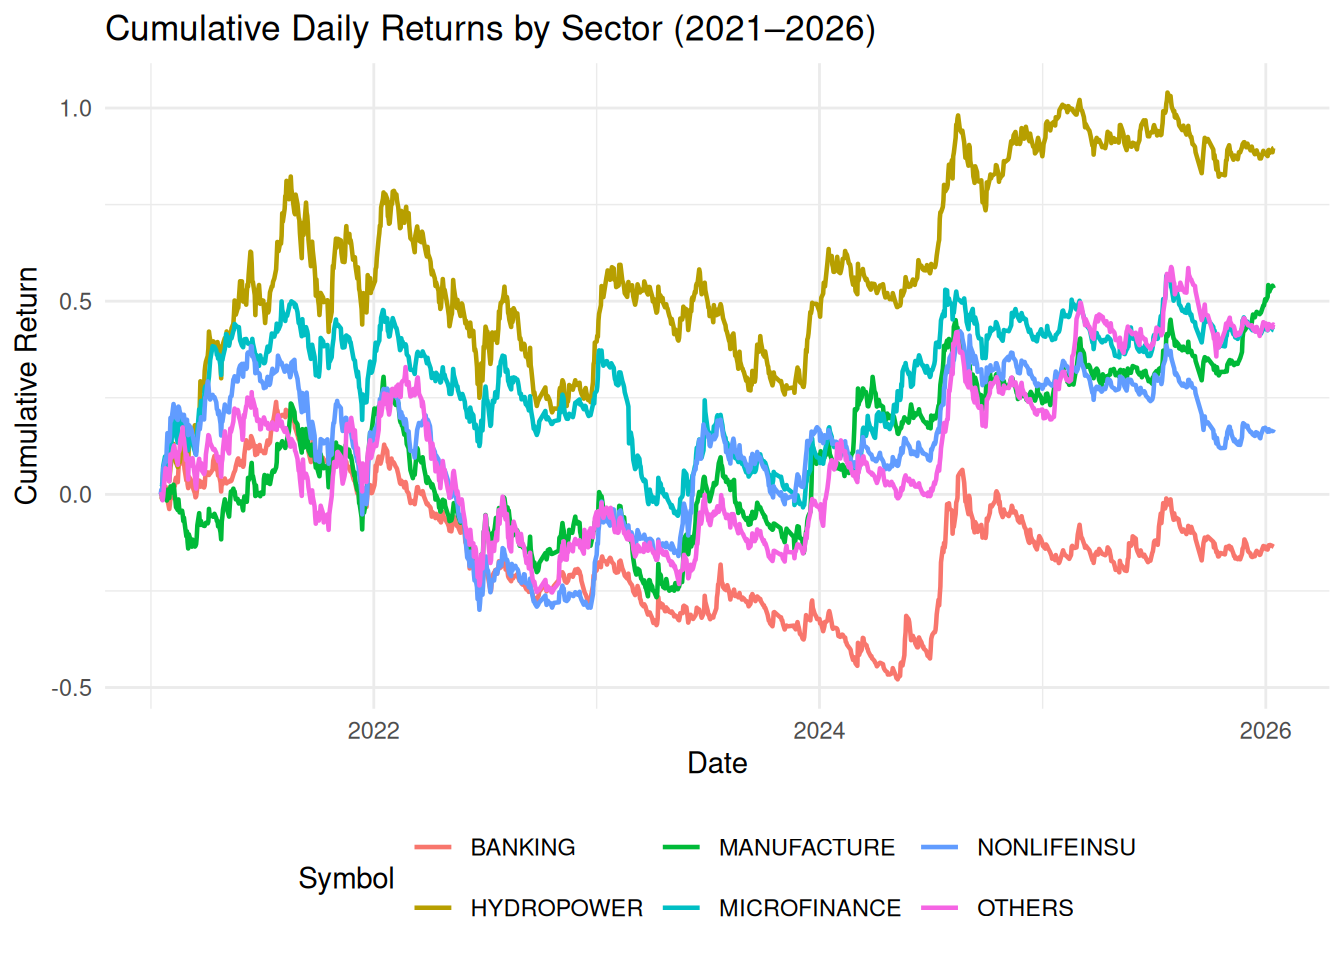
\includegraphics[width=\textwidth]{figures/stats-cumulative-ts.png}
\caption{Cumulative daily returns (2021--2026).}
\end{figure}
\column{0.48\textwidth}
\begin{figure}
\centering
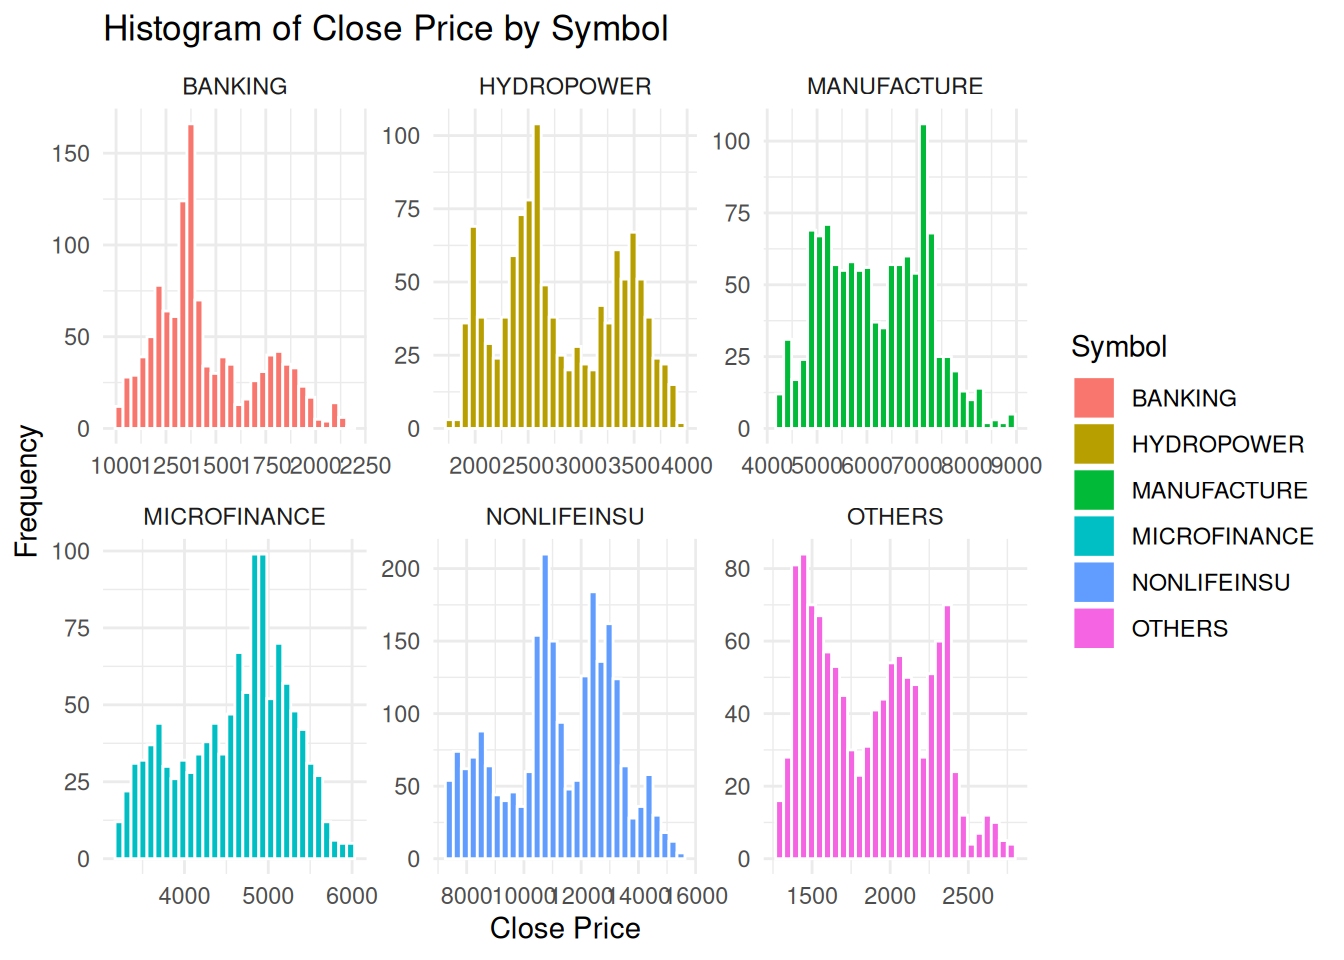
\includegraphics[width=\textwidth]{figures/stats-histogram.png}
\caption{Histogram of closing prices by sector.}
\end{figure}
\end{columns}
\begin{itemize}
    \item Hydropower shows strongest cumulative gain; Banking more modest.
    \item Histograms reveal right-skewed price distributions across sectors.
\end{itemize}
\end{frame}

% --- Slide 12: Confirmatory Tests ---
\begin{frame}{Month and Sector Effects -- Statistical Tests}
\begin{itemize}
    \item \textbf{Chi-square test} \cite{pearson1900chi}: Return direction (Gain/Loss) vs.\ month: $\chi^2(11)=92.578$, $p=5.2\times10^{-15}$ $\Rightarrow$ strong dependence.
    \item \textbf{One-way ANOVA (month)} \cite{fisher1925statistical}: $F=10.46$, $p<2\times10^{-16}$ $\Rightarrow$ significant monthly differences.
    \item \textbf{One-way ANOVA (sector)}: $F=0.497$, $p=0.779$ $\Rightarrow$ no significant sector differences.
    \item \textbf{Kruskal--Wallis (sector)} \cite{kruskal1952use}: $H=14.798$, $p=0.0113$ $\Rightarrow$ weak sector effect.
    \item \textbf{Mann--Whitney (Banking vs Others)} \cite{mann1947test}: $p=0.8648$ $\Rightarrow$ no difference.
\end{itemize}
\vspace{0.2cm}
\begin{block}{Takeaway}
Strong evidence for \textbf{monthly seasonality}; little evidence of persistent sectoral differences.
\end{block}
\end{frame}

% --- Slide 13: Best & Worst Months ---
\begin{frame}{Best and Worst Months}
\begin{columns}[T]
\column{0.48\textwidth}
\centering
\textbf{Two Best Months (by Mean Return)}
\smallskip
\scriptsize
\begin{tabular}{lccc}
\toprule
Sector & Month & Mean & Win\% \\
\midrule
BANKING      & Jul & 0.00599 & 60.2 \\
BANKING      & May & 0.00123 & 46.4 \\
HYDROPOWER   & Jan & 0.00653 & 59.4 \\
HYDROPOWER   & Jul & 0.00453 & 54.0 \\
MANUFACTURE  & Jul & 0.00488 & 62.8 \\
MANUFACTURE  & Dec & 0.00396 & 55.7 \\
MICROFINANCE & Jul & 0.00423 & 56.6 \\
MICROFINANCE & Jan & 0.00267 & 47.5 \\
NONLIFEINSU  & Jul & 0.00187 & 26.5 \\
NONLIFEINSU  & Jan & 0.00168 & 26.6 \\
OTHERS       & Jul & 0.00509 & 60.2 \\
OTHERS       & Jan & 0.00382 & 52.5 \\
\bottomrule
\end{tabular}
\column{0.48\textwidth}
\centering
\textbf{Two Worst Months}
\smallskip
\scriptsize
\begin{tabular}{lccc}
\toprule
Sector & Month & Mean & Win\% \\
\midrule
BANKING      & Aug & $-$0.00218 & 37.5 \\
BANKING      & Sep & $-$0.00179 & 36.7 \\
HYDROPOWER   & Sep & $-$0.00412 & 36.7 \\
HYDROPOWER   & Aug & $-$0.00210 & 40.4 \\
MANUFACTURE  & Aug & $-$0.00299 & 42.3 \\
MANUFACTURE  & Sep & $-$0.00184 & 35.6 \\
MICROFINANCE & Aug & $-$0.00287 & 36.5 \\
MICROFINANCE & Sep & $-$0.00274 & 38.9 \\
NONLIFEINSU  & Sep & $-$0.00199 & 18.9 \\
NONLIFEINSU  & Aug & $-$0.00136 & 18.8 \\
OTHERS       & Sep & $-$0.00469 & 32.2 \\
OTHERS       & Aug & $-$0.00300 & 31.7 \\
\bottomrule
\end{tabular}
\end{columns}
\vspace{0.15cm}
\small July dominates as the best month; August--September worst across all sectors.
\end{frame}

% --- Slide 14: Z-Score ---
\begin{frame}{Z-Score Entry/Exit Framework}
\begin{columns}[T]
\column{0.45\textwidth}
\begin{table}
\centering
\caption{\scriptsize ENTRY signals for Banking ($Z < -1.5$)}
\scriptsize
\begin{tabular}{lcc}
\toprule
Month & Freq. & Avg $Z$ \\
\midrule
January   & 4 & $-$2.24 \\
February  & 4 & $-$2.00 \\
March     & 3 & $-$1.90 \\
April     & 4 & $-$1.92 \\
May       & 6 & $-$2.03 \\
June      & 5 & $-$1.77 \\
July      & 5 & $-$1.84 \\
August    & 5 & $-$2.61 \\
September & 4 & $-$2.10 \\
October   & 4 & $-$1.83 \\
\bottomrule
\end{tabular}
\end{table}
\column{0.52\textwidth}
\begin{itemize}
    \item Z-score: $Z_{s,m,t} = \frac{R_{s,m,t} - \mu_{s,m}}{\sigma_{s,m}}$
    \item $|Z|>1.5$ flags extreme events \cite{tsay2010analysis}.
    \item $Z<-1.5$: oversold $\Rightarrow$ ENTRY signal.
    \item $Z>+1.5$: overbought $\Rightarrow$ EXIT signal.
    \item Average entry $Z \approx -2.0$ (two SD below monthly mean).
    \item Conservative threshold of $\pm 1.8$ recommended to reduce false signals given fat tails.
\end{itemize}
\end{columns}
\end{frame}

% --- Slide 15: Cumulative Return & Optimal Exit ---
\begin{frame}{Cumulative Return and Optimal Exit Day}
\begin{columns}[T]
\column{0.55\textwidth}
\begin{figure}
\centering
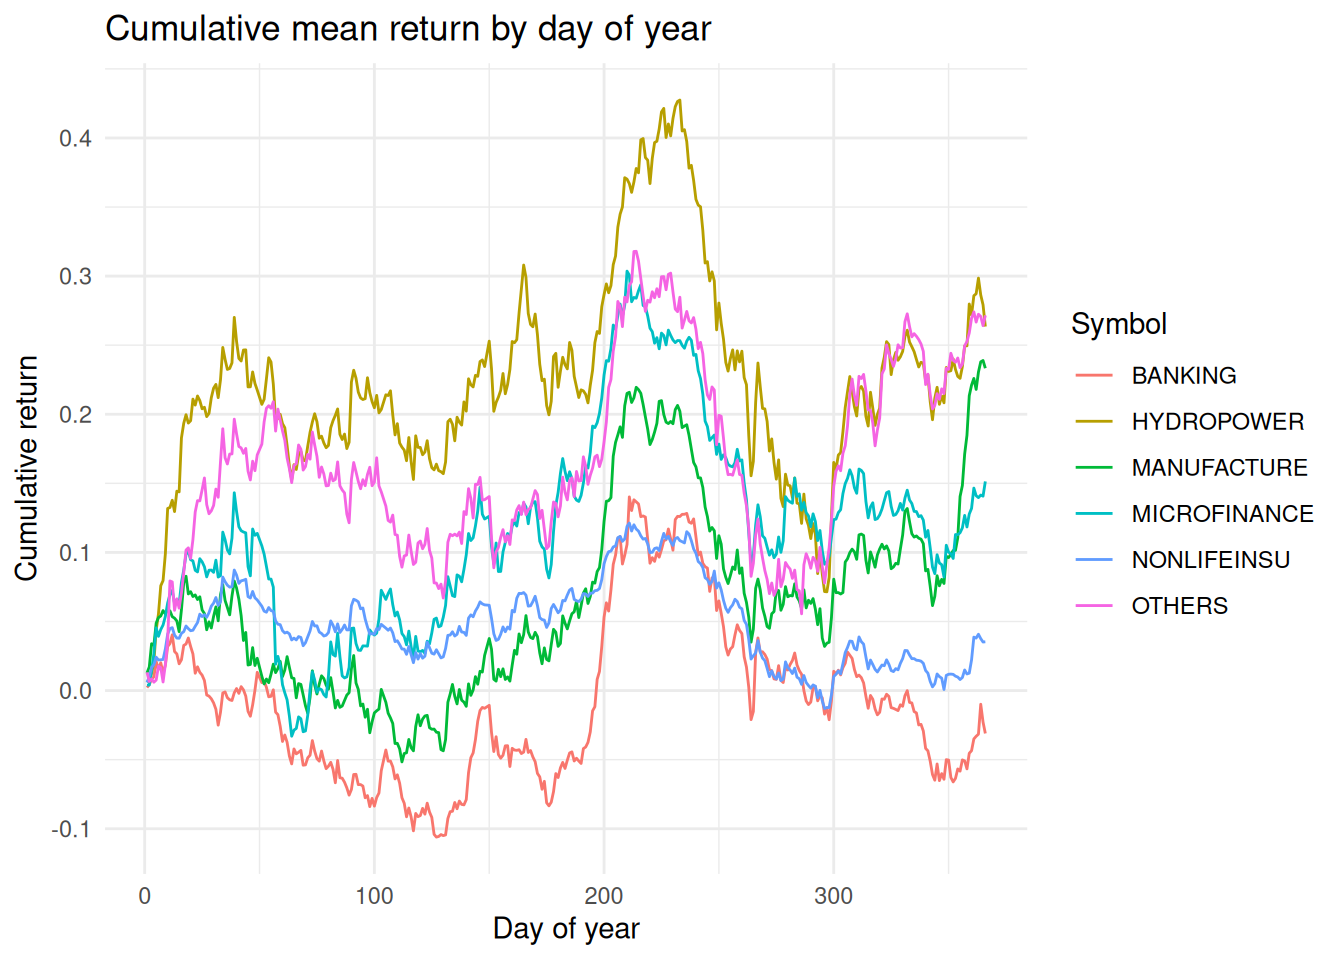
\includegraphics[width=\textwidth]{figures/stats-cumalative-return-by-year.png}
\caption{Cumulative mean return by day of year.}
\end{figure}
\column{0.42\textwidth}
\begin{table}
\centering
\caption{\scriptsize Optimal exit day \& cumulative return}
\scriptsize
\begin{tabular}{lcc}
\toprule
Sector & Exit Day & Cum.\ Ret. \\
\midrule
BANKING      & 210 (29 Jul)  & 0.113 \\
HYDROPOWER   & 230 (18 Aug)  & 0.422 \\
MANUFACTURE  & 365 (31 Dec)  & 0.202 \\
MICROFINANCE & 210 (29 Jul)  & 0.329 \\
NONLIFEINSU  & 210 (29 Jul)  & 0.120 \\
OTHERS       & 213 (1 Aug)   & 0.265 \\
\bottomrule
\end{tabular}
\end{table}
\end{columns}
\vspace{0.15cm}
\small Late July--early August is the optimal exit for most sectors; Hydropower peaks later (day 230).
\end{frame}

% --- Slide 16: Year-on-Year Consistency ---
\begin{frame}{Year-on-Year Consistency}
\begin{table}
\centering
\caption{Months with year-on-year consistency $\ge 0.80$ \cite{lakonishok1988seasonal}}
\small
\begin{tabular}{lccc}
\toprule
Sector & Month & Positive/Total Years & Consistency \\
\midrule
BANKING       & July     & 5/5  & 1.00 \\
HYDROPOWER    & January  & 6/6  & 1.00 \\
HYDROPOWER    & July     & 4/5  & 0.80 \\
HYDROPOWER    & November & 5/5  & 1.00 \\
MANUFACTURE   & January  & 5/6  & 0.833 \\
MANUFACTURE   & May      & 4/5  & 0.80 \\
MANUFACTURE   & July     & 4/5  & 0.80 \\
MICROFINANCE  & May      & 4/5  & 0.80 \\
MICROFINANCE  & July     & 4/5  & 0.80 \\
NONLIFEINSU   & May      & 4/5  & 0.80 \\
NONLIFEINSU   & July     & 4/5  & 0.80 \\
NONLIFEINSU   & November & 4/5  & 0.80 \\
OTHERS        & January  & 5/6  & 0.833 \\
OTHERS        & July     & 4/5  & 0.80 \\
OTHERS        & November & 5/5  & 1.00 \\
\bottomrule
\end{tabular}
\end{table}
\small July, January, and November are the most reliable months across sectors.
\end{frame}

% --- Slide 17: Bootstrap CIs ---
\begin{frame}{Bootstrap Confidence Intervals}
\begin{table}
\centering
\caption{95\% bootstrap percentile CIs for mean return in January \cite{efron1994introduction}}
\small
\begin{tabular}{lcc}
\toprule
Sector & Lower CI & Upper CI \\
\midrule
NONLIFEINSU  & 0.00005  & 0.00334 \\
MANUFACTURE  & $-$0.00170 & 0.00456 \\
BANKING      & $-$0.00238 & 0.00178 \\
OTHERS       & 0.00032  & 0.00730 \\
MICROFINANCE & $-$0.00012 & 0.00584 \\
HYDROPOWER   & 0.00263  & 0.01020 \\
\bottomrule
\end{tabular}
\end{table}
\begin{itemize}
    \item Hydropower and Others: CIs entirely above zero $\Rightarrow$ significant positive mean.
    \item Banking's interval straddles zero --- not statistically significant.
    \item Banking in August: CI $(-0.0048,\, 0.0004)$ includes zero, but direction uniformly negative.
\end{itemize}
\end{frame}

% --- Slide 18: Robust ANOVA + Permutation ---
\begin{frame}{Robust ANOVA and Permutation Test}
\begin{block}{Robust ANOVA (20\% trimmed means) \cite{wilcox2017introduction}}
$F_t = 12.2519$, $p < 0.001$, effect size $\hat{\eta} = 0.16$ (95\% CI $[0.13,\, 0.19]$) --- moderate-to-large.
\end{block}
\begin{itemize}
    \item Trimming removes extreme observations $\Rightarrow$ resistant to outliers and heterogeneity.
    \item Confirms month effect is \textbf{not} driven by a few extreme returns.
\end{itemize}
\vspace{0.3cm}
\begin{block}{Permutation Test (5000 shuffles) \cite{good2005permutation}}
$p < 2.2\times10^{-16}$ --- strongest distribution-free evidence of seasonality.
\end{block}
\begin{itemize}
    \item No distributional assumptions; provides the most robust validation.
    \item Together with robust ANOVA: monthly seasonality is a \textbf{genuine} feature, not an artifact.
\end{itemize}
\end{frame}

% --- Slide 19: Two-Way ANOVA + Summary ---
\begin{frame}{Two-Way Interaction ANOVA \& Summary of Key Findings}
\begin{columns}[T]
\column{0.45\textwidth}
\textbf{Two-Way ANOVA} \cite{kutner2005applied}
\begin{itemize}
    \item \textbf{Sector:} $F=0.502$, $p=0.775$ --- NS.
    \item \textbf{Month:} $F=10.44$, $p<2\!\times\!10^{-16}$ --- \textbf{highly significant}.
    \item \textbf{Sector$\times$Month:} $F=0.702$, $p=0.954$ --- NS.
\end{itemize}
$\Rightarrow$ Seasonal pattern is \textbf{uniform} across sectors.
\column{0.52\textwidth}
\textbf{Key Findings}
\begin{itemize}
    \item \textbf{July} is the premier month: highest returns, win ratios $>$60\%, perfect consistency (Banking).
    \item \textbf{Aug--Sep} are avoidance windows: negative returns, low win ratios, negative Sharpe ratios.
    \item \textbf{Optimal exit}: day 210--213 (late Jul--early Aug); Hydropower later (day 230).
    \item \textbf{Z-score}: avg entry $Z\approx -2.0$; threshold $\pm 1.8$ recommended.
    \item \textbf{Reliable}: July, January, November consistently positive across years.
\end{itemize}
\end{columns}
\end{frame}

% ===============================================================
%  SECTION 6: Conclusion  (Slide 20)
% ===============================================================
\section{Conclusion}

\begin{frame}{Conclusion}
\begin{enumerate}
    \item \textbf{Strong monthly seasonality} confirmed by multiple tests ($p<0.001$).
    \item \textbf{July is the optimal entry month} --- highest mean returns, win ratios, and consistency.
    \item \textbf{August--September are avoidance windows} --- uniformly negative returns.
    \item \textbf{Optimal exit:} late July--early August; Hydropower later, Manufacturing requires caution.
    \item \textbf{Z-score framework} provides actionable signals; conservative threshold recommended.
    \item \textbf{Sector-invariant pattern} --- a single seasonal calendar works for all sectors.
\end{enumerate}
\begin{block}{Practical Implication}
These findings challenge weak-form efficiency \cite{basnet2022efficient, joshi2025broad} and provide evidence-based timing rules for NEPSE investors \cite{gurung2024fiscal, adhikari2024calendar}.
\end{block}
\end{frame}

% ------------------- REFERENCES -------------------
\begin{frame}[allowframebreaks]{References}
\bibliographystyle{unsrt}
\bibliography{references}
\end{frame}

% ------------------- THANK YOU -------------------
\begin{frame}
\centering
\Huge \textbf{Thank You}
\vspace{1cm}

\large Questions \& Discussion
\end{frame}

\end{document}
